%
% pvfs2-client design
%

\documentclass[11pt]{article}
\usepackage[dvips]{graphicx}
\usepackage{times}

\graphicspath{{./}{figs/}} 

\pagestyle{plain}

\addtolength{\hoffset}{-2cm}
\addtolength{\textwidth}{4cm}

\addtolength{\voffset}{-1.5cm}
\addtolength{\textheight}{3cm}

\setlength{\parindent}{0pt}
\setlength{\parskip}{12pt}

\title{\texttt{pvfs2-client} Design Document (DRAFT)}
\author{PVFS Development Team}
\date{April 2003}

\begin{document}

\maketitle

\section{Introduction}

The primary role of the pvfs2-client daemon is to efficiently {\it
marshal} operation requests and data from the kernel's VFS ({\it
Virtual File System}, or {\it Virtual Filesystem Switch}) layer to
the pvfs2-server, and return responses from the pvfs2-server(s)
back to the VFS layer.  This involves waiting for file system and
I/O requests, performing operations against the  pvfs2-server
application(s), and passing responses back to the Linux kernel's VFS
layer.  The data medium for the communication between the VFS request
and the pvfs2-client application is the /dev/pvfs2 device node.  An
interface that will allow incoming unexpected requests from the
/dev/pvfs2 device node is required, and using the existing BMI
interface is preferred.

\begin{figure*}
\begin{center}
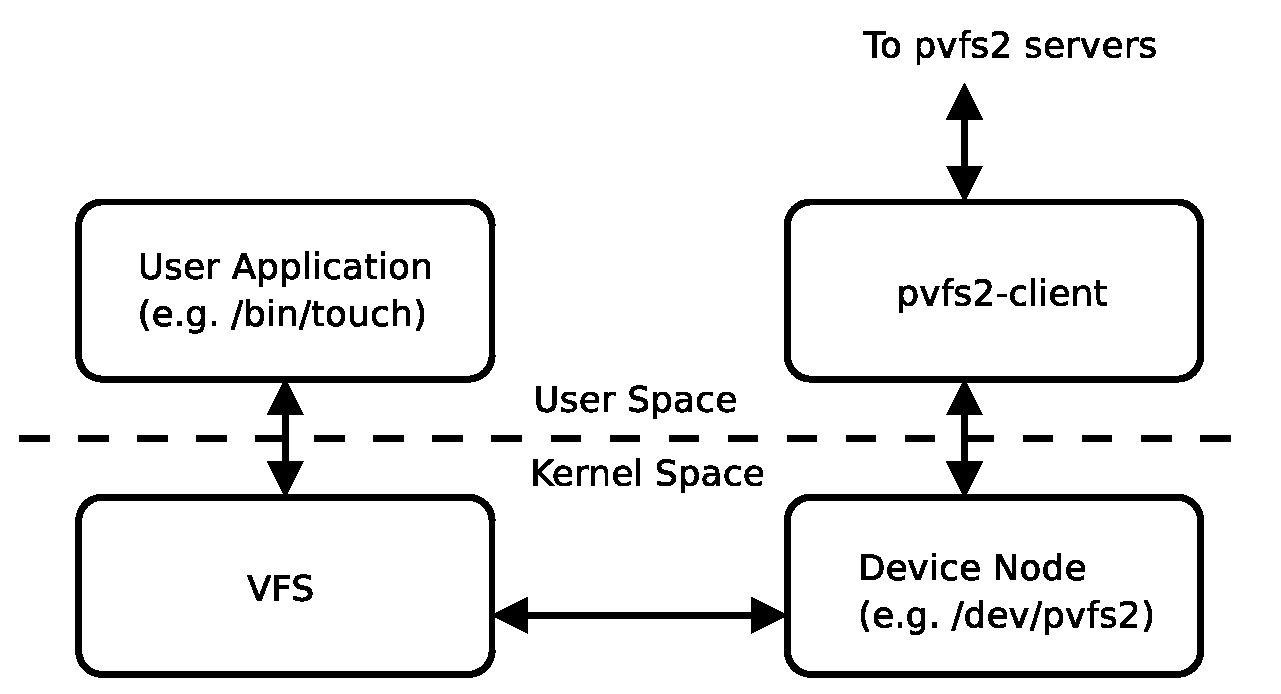
\includegraphics[scale=0.4]{pvfs2-vfs.eps}
\end{center}
\caption{High Level PVFS2 Architecture}
\label{figure:arch}
\end{figure*}

Figure 1 illustrates the architecture of several components of
PVFS2.  This document will focus specifically on the pvfs2-client
application.

\section{Motivation for the \texttt{pvfs2-client} Application}

Currently, our entire code base exists as user space code.  This
includes all of our networking support (through the {\it BMI} and {\it
Flow Interfaces}), and our non-blocking request handling architecture
through the {\it Job Interface}.  The pvfs2-server already uses these
interfaces to manage multiple simultaneous operations in flight at
once.  Similarly, it is highly desirable to have a pvfs2-client
application that can issue and manage multiple simultaneous operations
at once when communicating with the pvfs2-servers.  Therefore, at least
in the short term, it would be most appropriate to leverage as much of
our existing code as possible.  A user-space application is required
to make use of this code, and thus the need for the pvfs2-client
application to bridge the gap between the Linux kernel's VFS layer and
the {\it System Interface}.

\section{\texttt{pvfs2-client} Application Architecture}

The pvfs2-client application consists of a set of state machines
roughly corresponding to all file system and I/O operations that can
be requested from the VFS.  At a high level, the pvfs2-client
application appears to share a common architecture with the
pvfs2-server application.  The most notable distinction between the
pvfs2-client architecture and the pvfs2-server architecture is the
source of the unexpected requests.  On the pvfs2-server, unexpected
requests come from over the network through the BMI Interface.  The
pvfs2-client receives unexpected messages from the /dev/pvfs2 device
node.  It would be ideal if the BMI Interface could be used to monitor
the /dev/pvfs2 device node.

One responsibility of the pvfs2-client application is to wait for jobs
in progress to complete.  Waiting on pending jobs is implemented as a
non-blocking operation against the existing job interface using the
call job\_testcontext.  This call returns a list of unexpected or
completed jobs that were submitted previously by states of the various
state machine operation implementations.

For each job returned from job\_testcontext, the pvfs2-client
application checks if the job is an unexpected request.  If the
job {\it is} an unexpected request, it initializes an appropriate
state machine for that job.  Regardless of whether or not the job was
unexpected, the state of each job is advanced to the next until a
blocking operation is encountered.

Unexpected requests are delivered to the pvfs2-client application only
from the /dev/pvfs2 device node that the pvfs2-client application
monitors through the job interface.  These requests are generated and
passed up from the Linux kernel's VFS layer by the PVFS2 kernel module
that implements the VFS operations.

The pvfs2-client has a similar processing loop as the pvfs2-server:

\begin{verbatim}
    while (pvfs2-client application is running)
    {
      ...
      wait on pending jobs in progress and expected requests
      ...
      foreach job returned
         if job is an unexpected request
            initialize appropriate operation state machine
         end if
         ...
         while completions occur immediately
             advance to next state in state machine
         end while
      end foreach
    }
\end{verbatim}

\section{Limitations of the Existing System Interface}

Currently, all client interaction to a pvfs2-server is done through
the {\it System Interface} API.  This interface provides a set of file
system and I/O operations to be performed against the pvfs2-server(s),
but suffers from several major limitations in its current state.
These limitations can be described briefly as:

\begin{itemize}
  \item \emph{Semantic Limitations}: the current implementation
    provides a blocking interface to all operations.  We already know
    that a non-blocking interface is required for efficient access
    through other existing non-blocking iterfaces such as ROMIO.
  \item \emph{Reusability Limitations}: the current implementation
    performs many blocking operations.  This cannot be used {\it as
    is} in the proposed non-blocking state-machine oriented
    architecture of the pvfs2-client.
\end{itemize}

A proposed redesign of the System Interface implemented in terms of
reusable state machines can solve these limitations, as discussed
below.

\section{\texttt{pvfs2-client} Request Servicing}

\begin{figure*}
\begin{center}
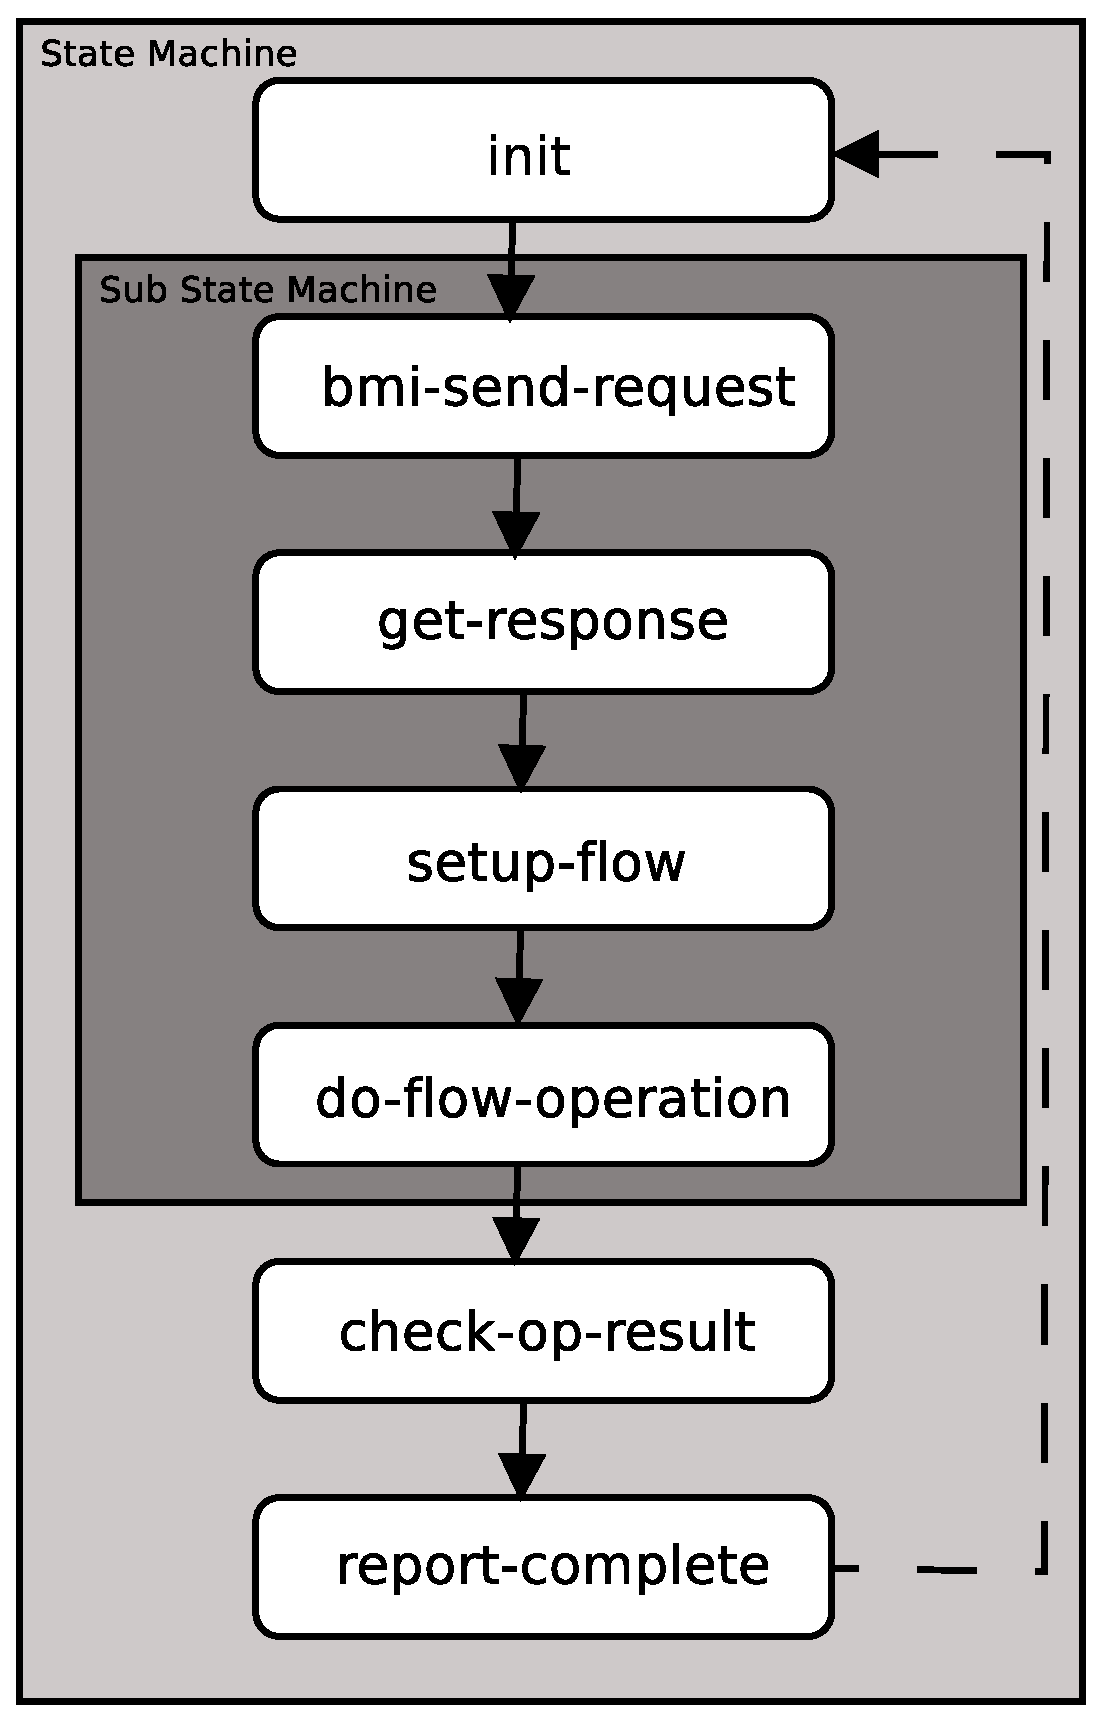
\includegraphics[scale=0.4]{core-sm.eps}
\end{center}
\caption{Operation Servicing State Machine (w/nested core state machine)}
\label{figure:generic-sm}
\end{figure*}

Operation request servicing in the pvfs2-client application will be
implemented by state machines.  That is, for each type of request that
can be handed up from the PVFS2 kernel module, a matching state
machine will exist to service it.  The types of operation requests
required will roughly correspond to all of the possible operations
available through the System Interface API.  For the proposed
pvfs2-client architecture, it is clear that a non-blocking
implementation of the System Interface is desirable for the state
machine architecture.  Further, to encourage code re-use, each
operation in the {\it System Interface} can be expressed as a state
machine.  Implementing the core functionality of the System Interface
methods in terms of state machines allows an opportunity for blocking
{\it and} non-blocking interface implementations, heavier code re-use,
and design simplicity.

We can think of all pvfs2-client operations as having a similar
structure, as depicted in Figure 2.  What we see here is a generic
state machine implementing an operation.  For all operations there
will be a {\it use specific} initialization, execution of some core
routines (i.e. functionality provided by the current System
Interface), and a use-specific notification of status and completion.
If the core functionality of each System Interface routine were
implemented in terms of a state machine, the execution of a core
routine could be embedded as a nested state machine within the
operation specific state machine.

Figure 2 shows a complete operation state machine, along with the
embedded (nested) state machine that implements core functionality of
a System Interface call.  The first state called {\it init} represents
the use specific initialization state.  Each operation may have a
different initialization phase, but at the very least, the source and
target endpoints for the Flow (to be performed inside the nested state
machine) are selected.  Following initialization, the nested state
machine is executed, performing the core operation requested.  After
this, the operation state machine checks the status of the performed
operation to properly handle error reporting.  Finally, the state is
advanced to the initial state of the state machine, which is the
default action when the operation has completed.

In order to represent the core functionality of a System Interface
method as a re-useable state machine, we must take advantage of the
source and target endpoint specifications allowed by the existing {\it
Flow Interface}.  Assuming it is possible to know the source and
target endpoints of the Flow prior to executing the System Interface
core functionality, it can be re-used by embedding it as a nested
state machine in the pvfs2-client architecture, {\it and} shared
between the blocking and non-blocking System Interface
implementations.  The requirement for this is that the source and
target endpoints of the Flow be established before using the core
functionality state machine.  In Figure 2, for example, the
pvfs2-client application may specify that the Flow's target endpoint
should be the /dev/pvfs2 device node.

\section{Non-blocking and Blocking System Interface Implementations}

Non-blocking and blocking System Interface methods (as shown in Figure
3) can use the same core functionality once implemented as a state
machine.  The blocking version will manually advance the state machine
internal to the call and not return until the operation has completed.
The non-blocking implementation will start the state machine and offer
a mechanism for testing operation completion.  For the non-blocking
interface, some method of asynchronous progress must be provided.
This can be done either with a background thread, or completing work
during a test for completion.

\end{document}
